\subsection{Klassendiagramm}
Die Klassen der Software arbeiten nach dem folgenden Klassendiagramm.
\begin{figure}[H]
    \centering
    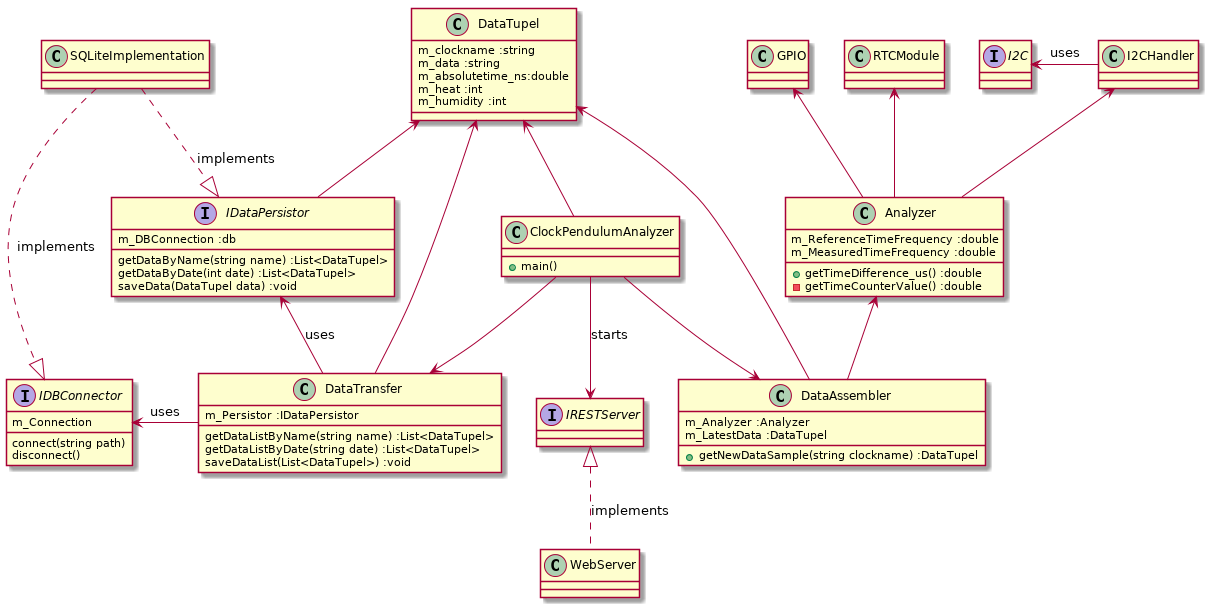
\includegraphics[width=.7\textwidth]{classdiagramm.png}
    \caption{Klassendiagramm der C++ Software auf dem Raspberry Pi}
\end{figure}
\subsubsection{Klassdetails}
    %TODO subject to change
	\begin{description}
        \item[I2CHandler] Diese Klasse öffnet und schliesst den $I^2C$-Bus und liest Daten von daran angeschlossenen Geräten.
        \item[GPIO] Eine Klasse die für das Arbeiten mit GPIO Pins auf dem Raspberry Pi zuständig ist.
        \item[Analyzer] Die Klasse ist für die Berechnung der Zeitdifferenz in Nanosekunden zuständig. Es kann auch die Differenz in Mikro- und Millisekunden ausgegeben werden.
    \end{description}